\documentclass[smaller]{beamer}
\usepackage[utf8]{inputenc}
\usepackage{polski}
% \usepackage{color}
\usepackage{transparent}
\usepackage{amsrefs}
\usepackage{amsfonts}
\usepackage{listings}
\usepackage{syntax}
\usepackage{wrapfig}
\usepackage{graphicx}
\usepackage{caption}
\usepackage{subcaption}

\graphicspath{{includes/}}

\definecolor{javared}{rgb}{0.6,0,0} % for strings
\definecolor{javagreen}{rgb}{0.25,0.5,0.35} % comments
\definecolor{javapurple}{rgb}{0.5,0,0.35} % keywords
\definecolor{javadocblue}{rgb}{0.25,0.35,0.75} % javadoc

 \lstloadlanguages{
         Java
 }
 \lstset{language=Java,
%          basicstyle=\footnotesize\ttfamily, % Standardschrift
         basicstyle=\footnotesize\ttfamily, % Standardschrift
         %numbers=left,               % Ort der Zeilennummern
         numberstyle=\tiny\color{black},          % Stil der Zeilennummern
         stepnumber=1,               % Abstand zwischen den Zeilennummern
         numbersep=5pt,              % Abstand der Nummern zum Text
         tabsize=3,                  % Groesse von Tabs
% 	inputencoding=utf8, extendchars=\true
         extendedchars=true,         %
         breaklines=true,            % Zeilen werden Umgebrochen
keywordstyle=\color{javapurple}\bfseries,
stringstyle=\color{javared},
commentstyle=\color{javagreen},
morecomment=[s][\color{javadocblue}]{/**}{*/},
    		frame=b,         
 %        keywordstyle=[1]\textbf,    % Stil der Keywords
 %        keywordstyle=[2]\textbf,    %
 %        keywordstyle=[3]\textbf,    %
 %        keywordstyle=[4]\textbf,   \sqrt{\sqrt{}} %
         stringstyle=\color{blue}\ttfamily, % Farbe der String
         showspaces=false,           % Leerzeichen anzeigen ?
         showtabs=false,             % Tabs anzeigen ?
         xleftmargin=10pt,
         framexleftmargin=10pt,
         framexrightmargin=5pt,
         framexbottommargin=4pt,
         %backgroundcolor=\color{lightgray},
         showstringspaces=false      % Leerzeichen in Strings anzeigen ?        
 }
    %\DeclareCaptionFont{blue}{\color{blue}} 

  %\captionsetup[lstlisting]{singlelinecheck=false, labelfont={blue}, textfont={blue}}
  \usepackage{caption}
\DeclareCaptionFont{white}{\color{white}}
\DeclareCaptionFormat{listing}{\colorbox[cmyk]{0.43, 0.35, 0.35,0.01}{\parbox{\textwidth}{\hspace{15pt}#1#2#3}}}
\captionsetup[lstlisting]{format=listing,labelfont=white,textfont=white, singlelinecheck=false, margin=0pt, font={bf,footnotesize}}


\usetheme{Warsaw}
\title[Złożone architektury - implementacja]{Złożone architektury bez podziału na warstwy.}
\author{Paweł Cesar Sanjuan Szklarz}
\institute{Confitura 2012}
\date{30 czerwca 2012}
\begin{document}

\begin{frame}
\titlepage
\end{frame}

% \begin{frame}
%  \tableofcontents
% \end{frame}

\section{Warstwy}
\subsection{Warstwy są mało efektywne}

\begin{frame}{Plan}
Plan:
\begin{description}
 \item[od] \hfill \\
 Warstwy $\Rightarrow$ Porządek $\Rightarrow$ Złożone systemy
 \item[do] \hfill \\
 Inject $\Rightarrow$ Architektura $\Rightarrow$ Złożone systemy
\end{description}
\end{frame}

\begin{frame}{Warstwy???}
 \begin{figure}
 \centering
 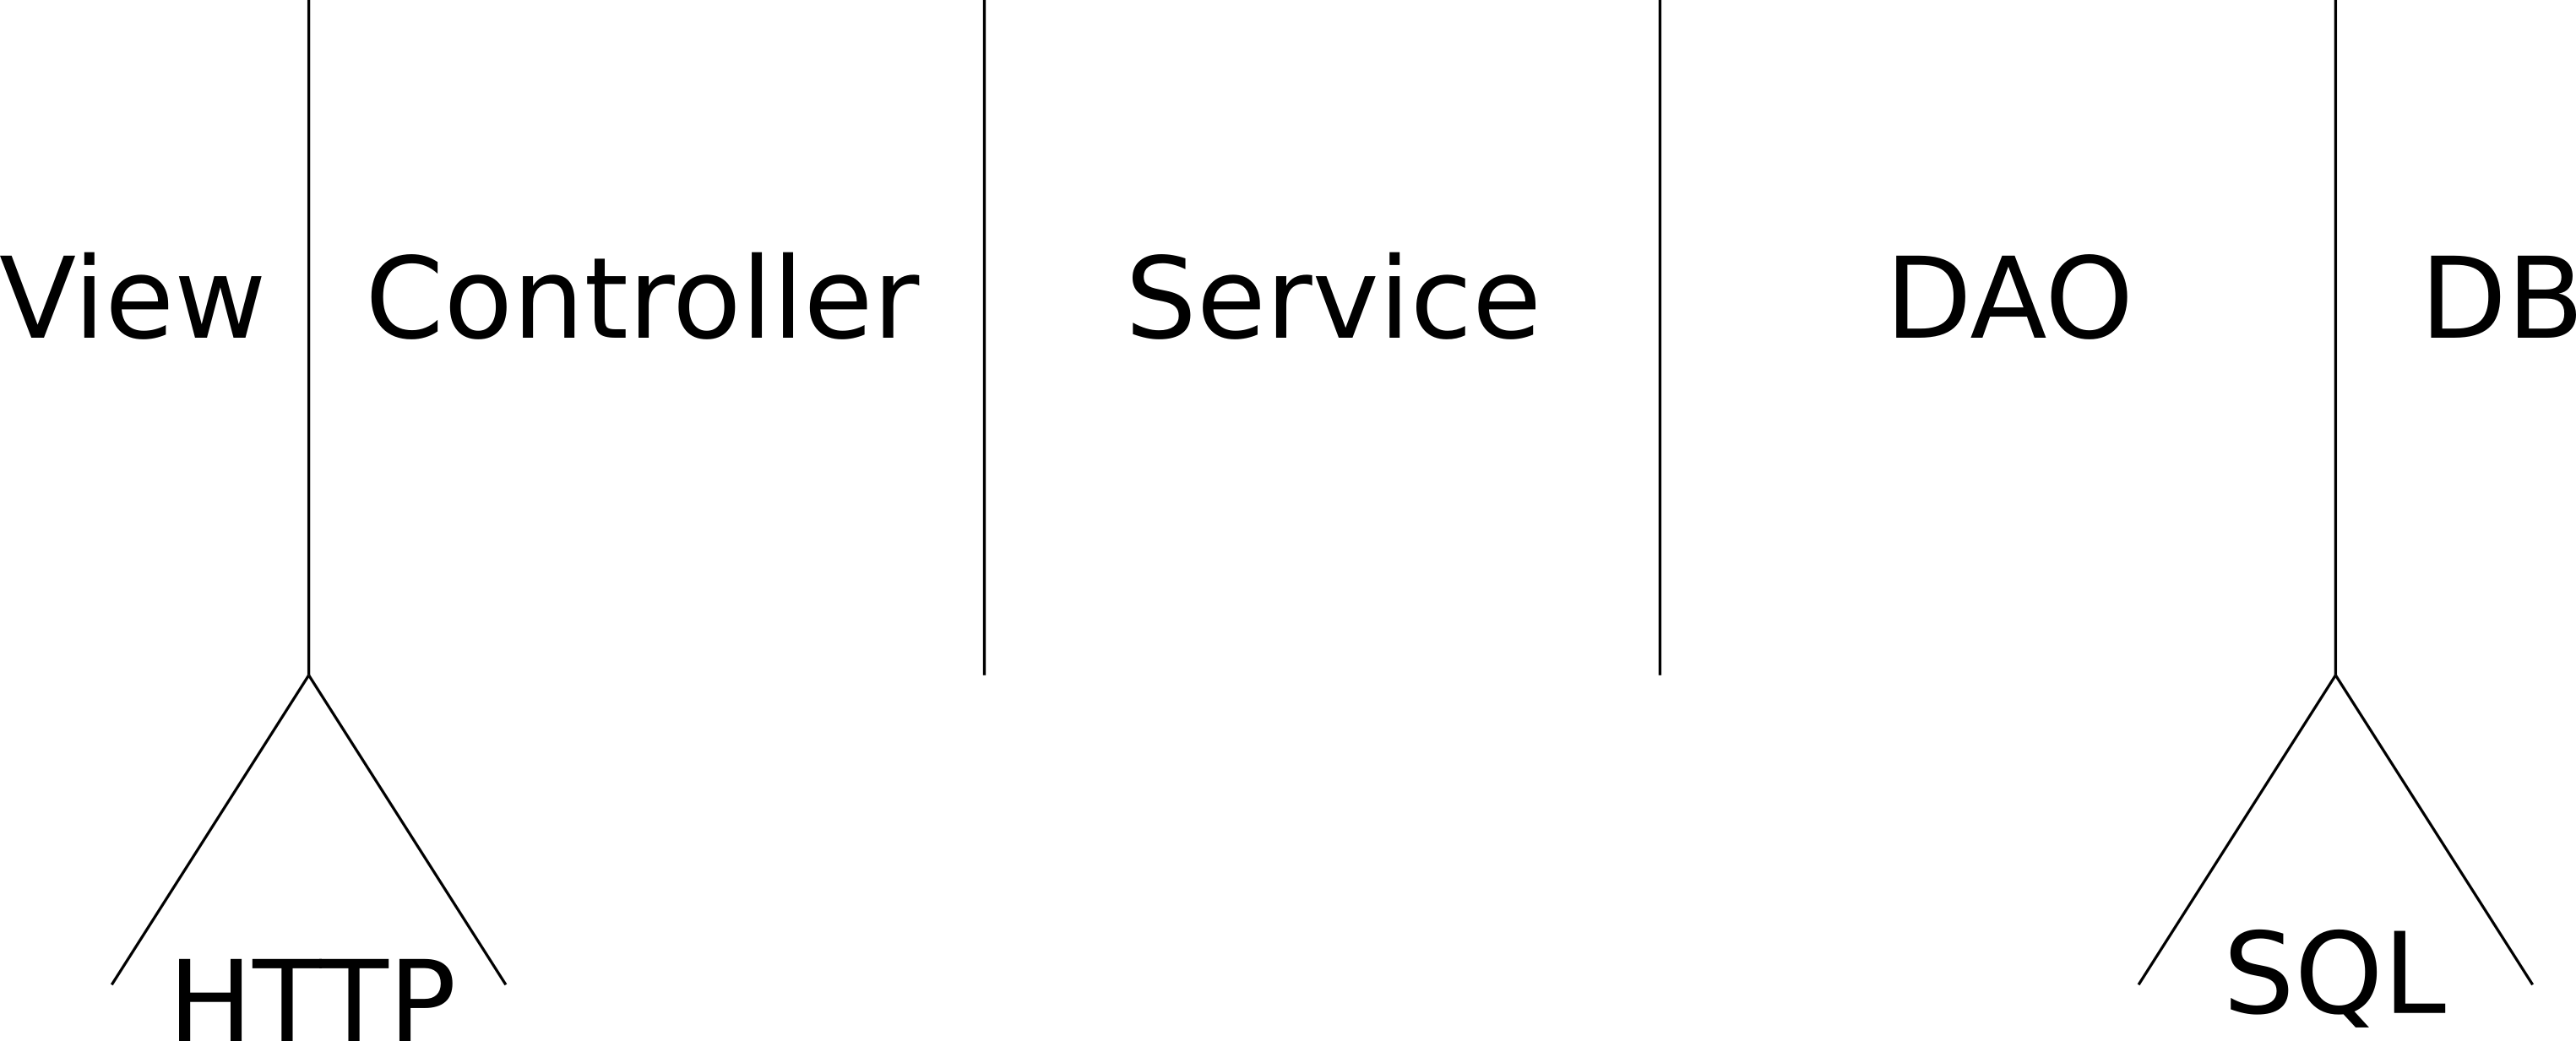
\includegraphics[width=1\textwidth]{3warstwyFig}
\end{figure}
\end{frame}

\begin{frame}{Za dużo warstw}
\begin{figure}
 \centering
 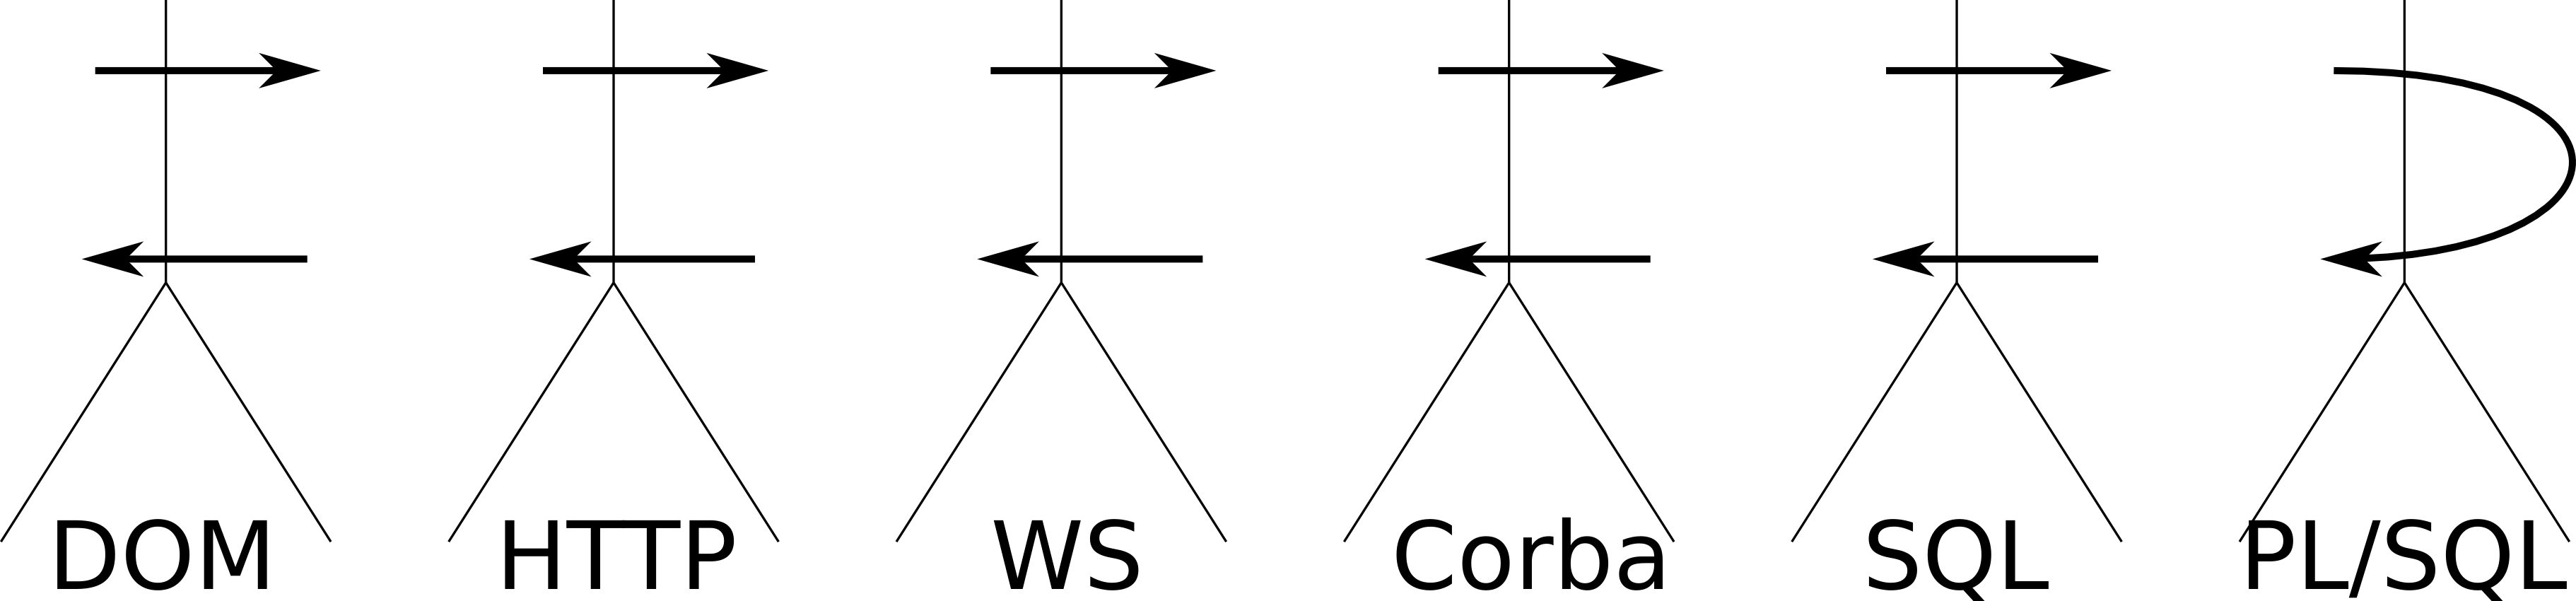
\includegraphics[width=1\textwidth]{duzoWarstwFig}
\end{figure}
\end{frame}

\subsection{Demo}
\begin{frame}{Demo}
 Logika wywołań pomiędzy warstwami.
\end{frame}

\defverbatim[colored]\LstLogicDrop{%
\begin{lstlisting}[tabsize=2,frame=single]
public class Controller {
	private Service service;
	void operation(String args) {
		service.operation(args);
	}
}

public class Service {
	private DAO dao;
	void operation(String args) {
		dao.operation(args);
	}
}

public class DAO {
	private DB db;
	void operation(String args) {
		// logic
	}
}
\end{lstlisting}}

\subsection{Problemy}
\begin{frame}{Wymuszenie na logikę w kodzie}
\LstLogicDrop
\end{frame}

\begin{frame}{Ubogie przekazanie kontekstu}
 ``\lstinline|service.operation(args)|'' : args  $\Rightarrow$ kontekst
\pause
\begin{figure}
 \centering
 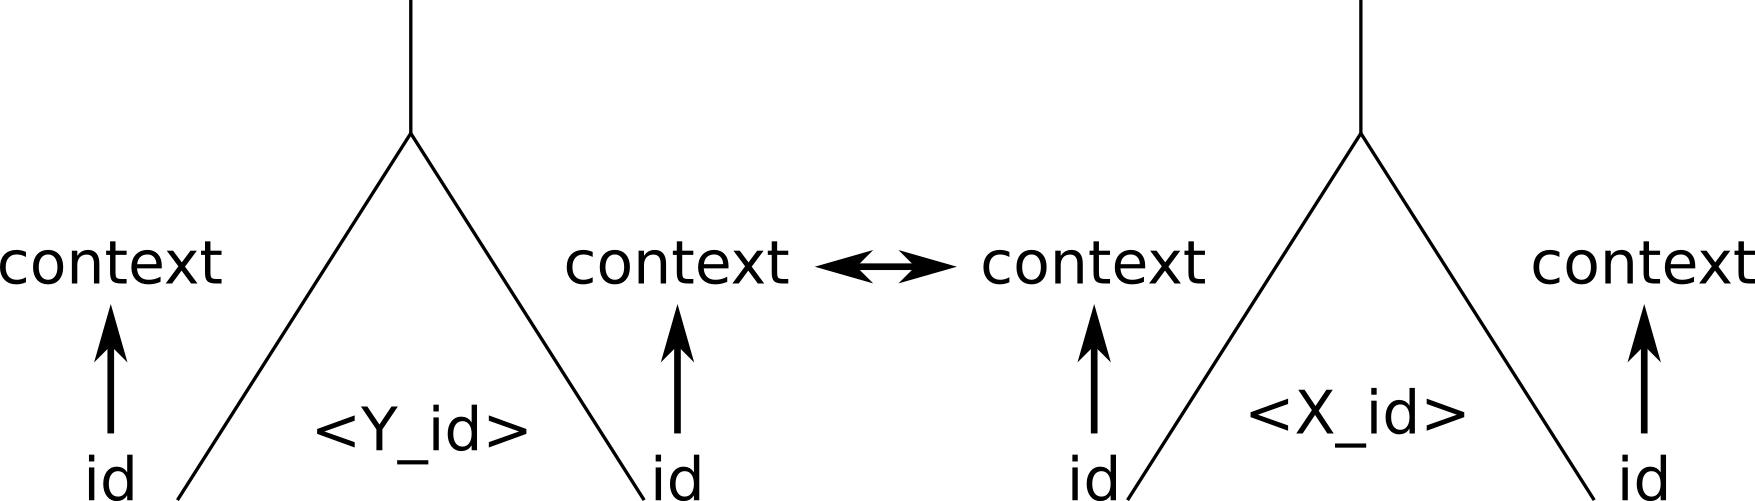
\includegraphics[width=1\textwidth]{contextMapFig}
\end{figure}
\end{frame}

\defverbatim[colored]\LstLogicGarbage{%
\begin{lstlisting}[tabsize=2,frame=single]
A {
	Data logicParameter = B.extractData(...);
	C.businessOperation(logicParameter);
}
\end{lstlisting}}

\begin{frame}{Zaśmiecenie logiki}
\LstLogicGarbage


\begin{figure}
 \centering
 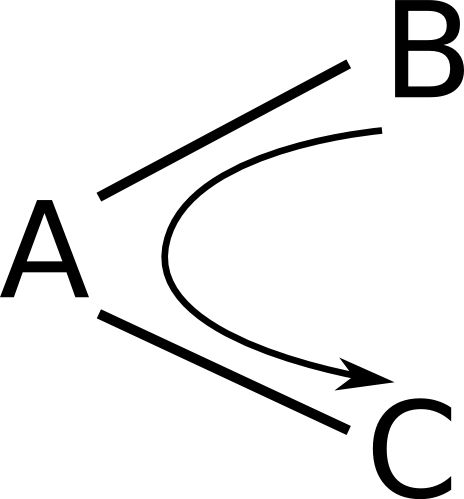
\includegraphics[width=.3\textwidth]{logicGarbageSimpleFig}
\end{figure}

\end{frame}

\begin{frame}{PASKUDNE!!! zaśmiecenie logiki}
\begin{figure}
 \centering
 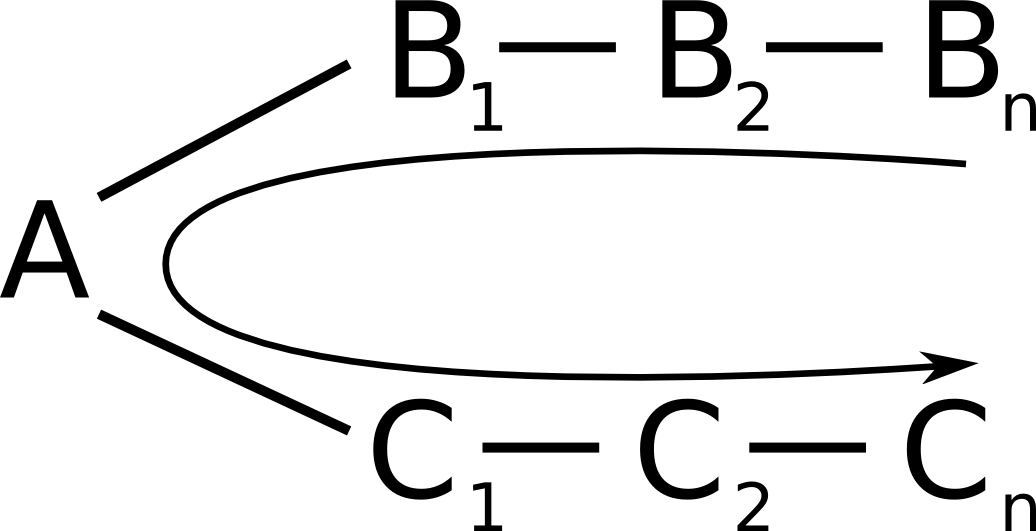
\includegraphics[width=1\textwidth]{logicGarbageComplexFig}
\end{figure}

\end{frame}

\begin{frame}{Pozornie wyróżniony kierunek}
\begin{figure}
 \centering
 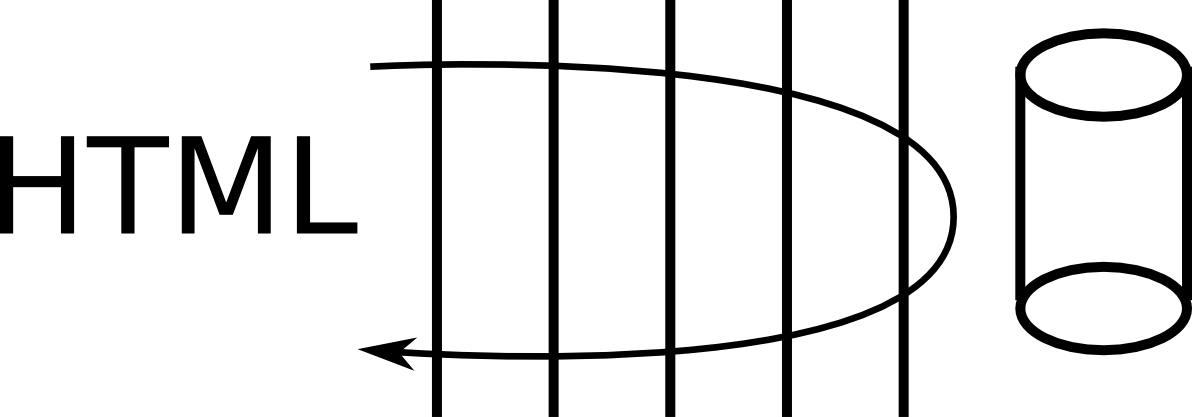
\includegraphics[width=1\textwidth]{pozornyKierunekFig}
\end{figure} 
\end{frame}

\subsection{Ciekawostka}
\begin{frame}{Ciekawostka}
 2d: Obrót + przesunięcie = Obrót
\begin{figure}
 \centering
 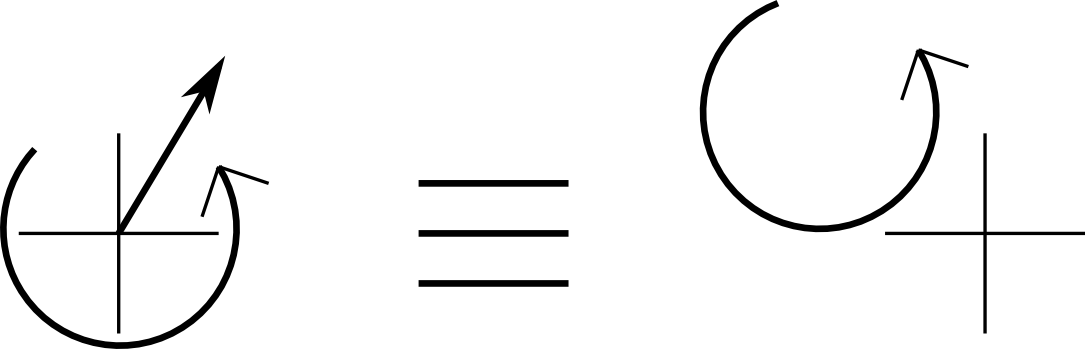
\includegraphics[width=1\textwidth]{rotation2dFig}
\end{figure}
\end{frame}

\begin{frame}{Dowód}
$$(O_1 O_2 ) (O_2 O_3) = O_1 O_3 $$

\begin{figure}
 \centering
 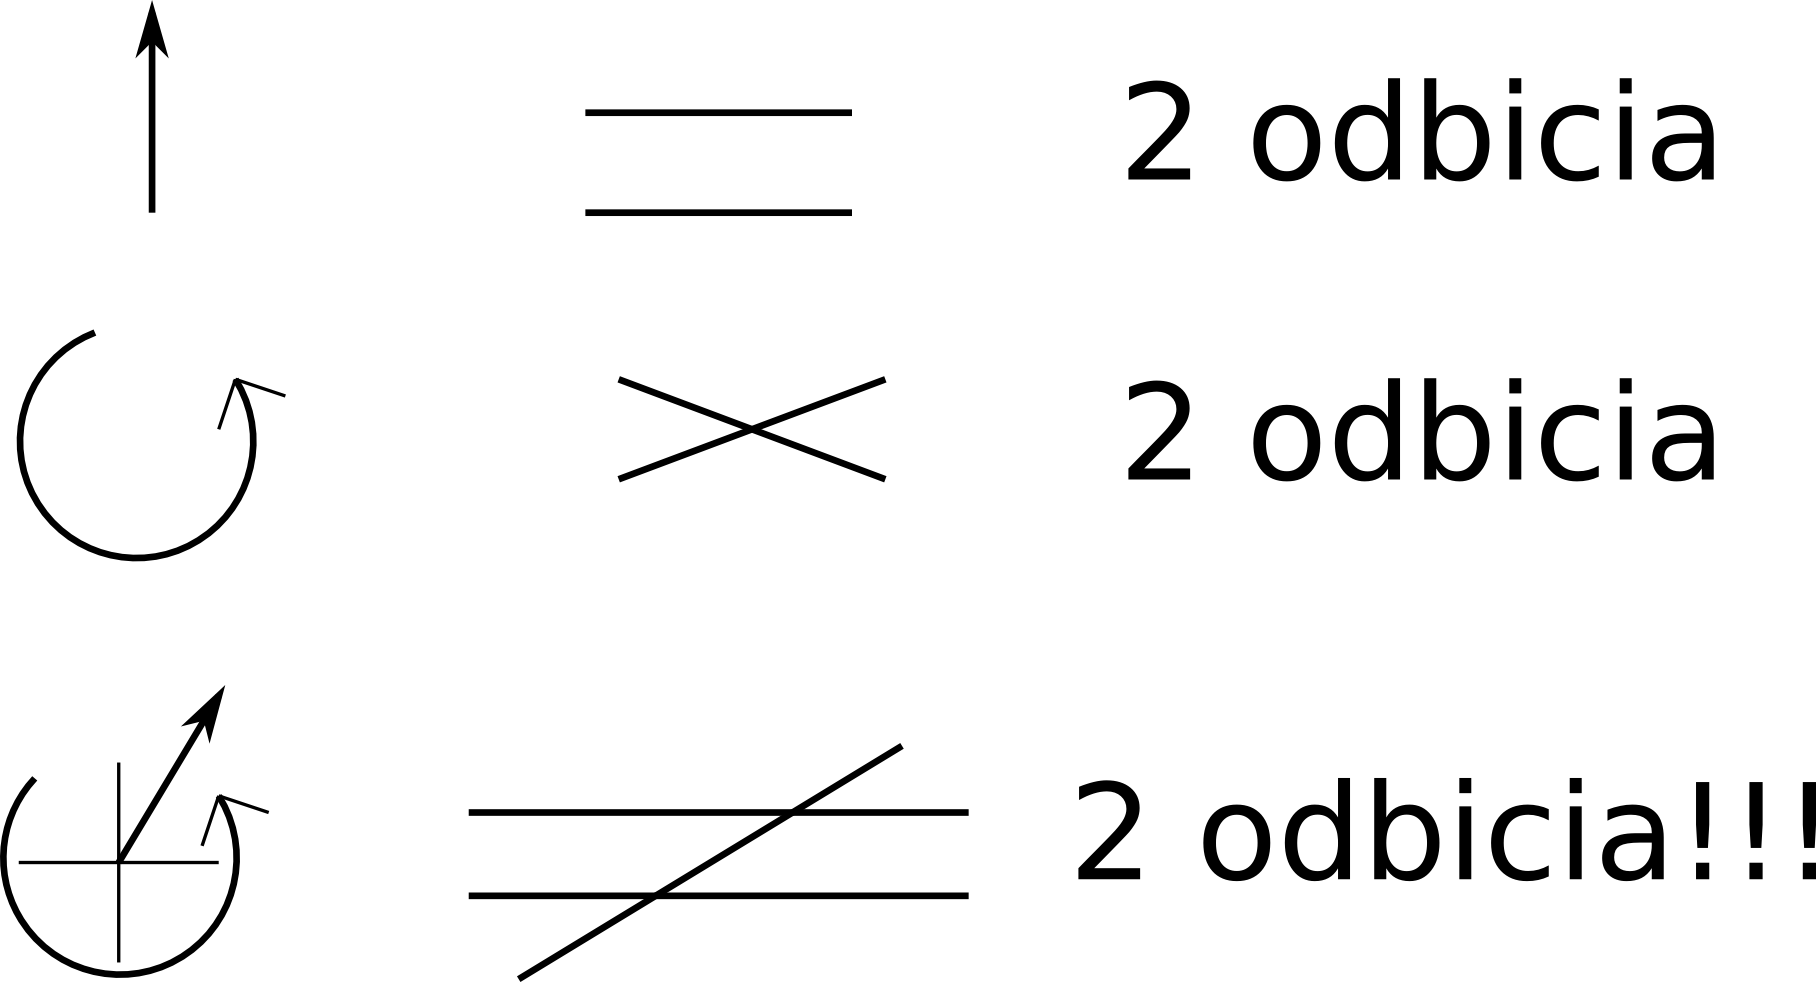
\includegraphics[width=1\textwidth]{rotationDowodFig}
\end{figure}

\end{frame}

\section{Inject - Architektura}
\subsection{Demo}

\begin{frame}{Demo}
 DEMO
\end{frame}


\defverbatim[colored]\LstSimpleInjection{%
\begin{lstlisting}[tabsize=2,frame=single]
class A {
	@Inject private Service service;
}
class B implements Service {}
\end{lstlisting}}

\subsection{Propozycja - SAM}
\begin{frame}{Zdalne injektowanie zależności}
\LstSimpleInjection
\pause

\begin{figure}
 \centering
 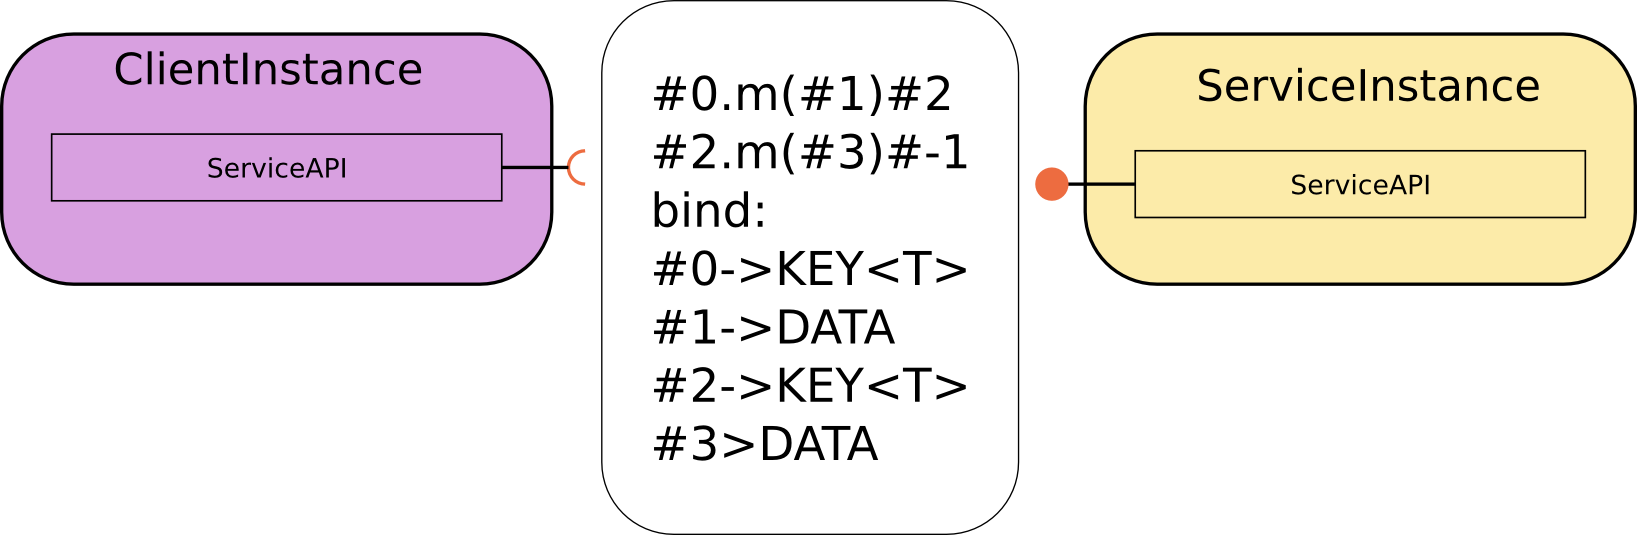
\includegraphics[width=1\textwidth]{canonicalSplit}
\end{figure}

\end{frame}

\defverbatim[colored]\LstLogicDropSolution{%
\begin{lstlisting}[tabsize=2,frame=single]

class client {
	@Inject private PublicAPI service;
}

interface PublicAPI {
}

class ServiceImplementation implements InternalAPI {
}
interface InternalAPI extends PublicAPI {
}

\end{lstlisting}}

\subsection{Rozwiązania}
\begin{frame}{Problem - Wymuszenie na logiki w kodzie}

\LstLogicDropSolution

\end{frame}


\begin{frame}{Problem - Ubogie przekazanie kontekstu}
\begin{figure}
 \centering
 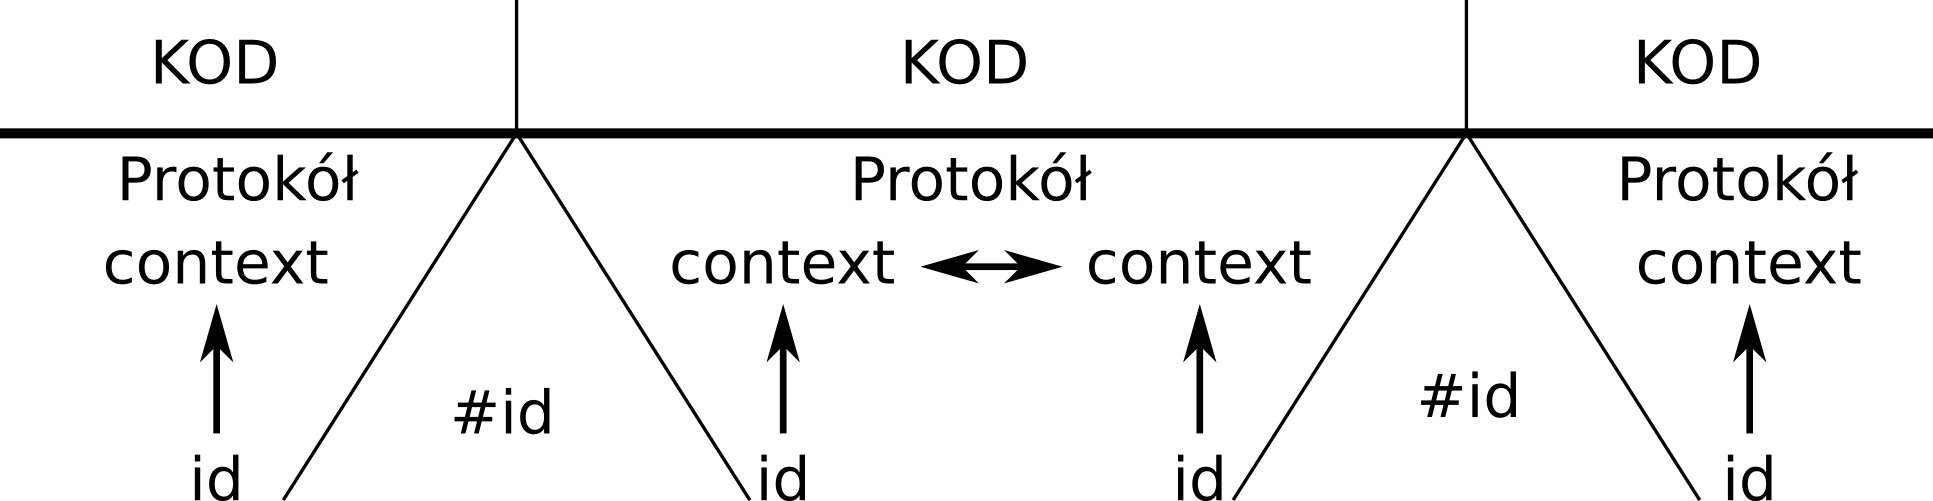
\includegraphics[width=1\textwidth]{contextMapSolutionFig}
\end{figure}
\end{frame}

\begin{frame}{Problem - Zaśmiecenie logiki}
\LstLogicGarbage

\begin{figure}
 \centering
 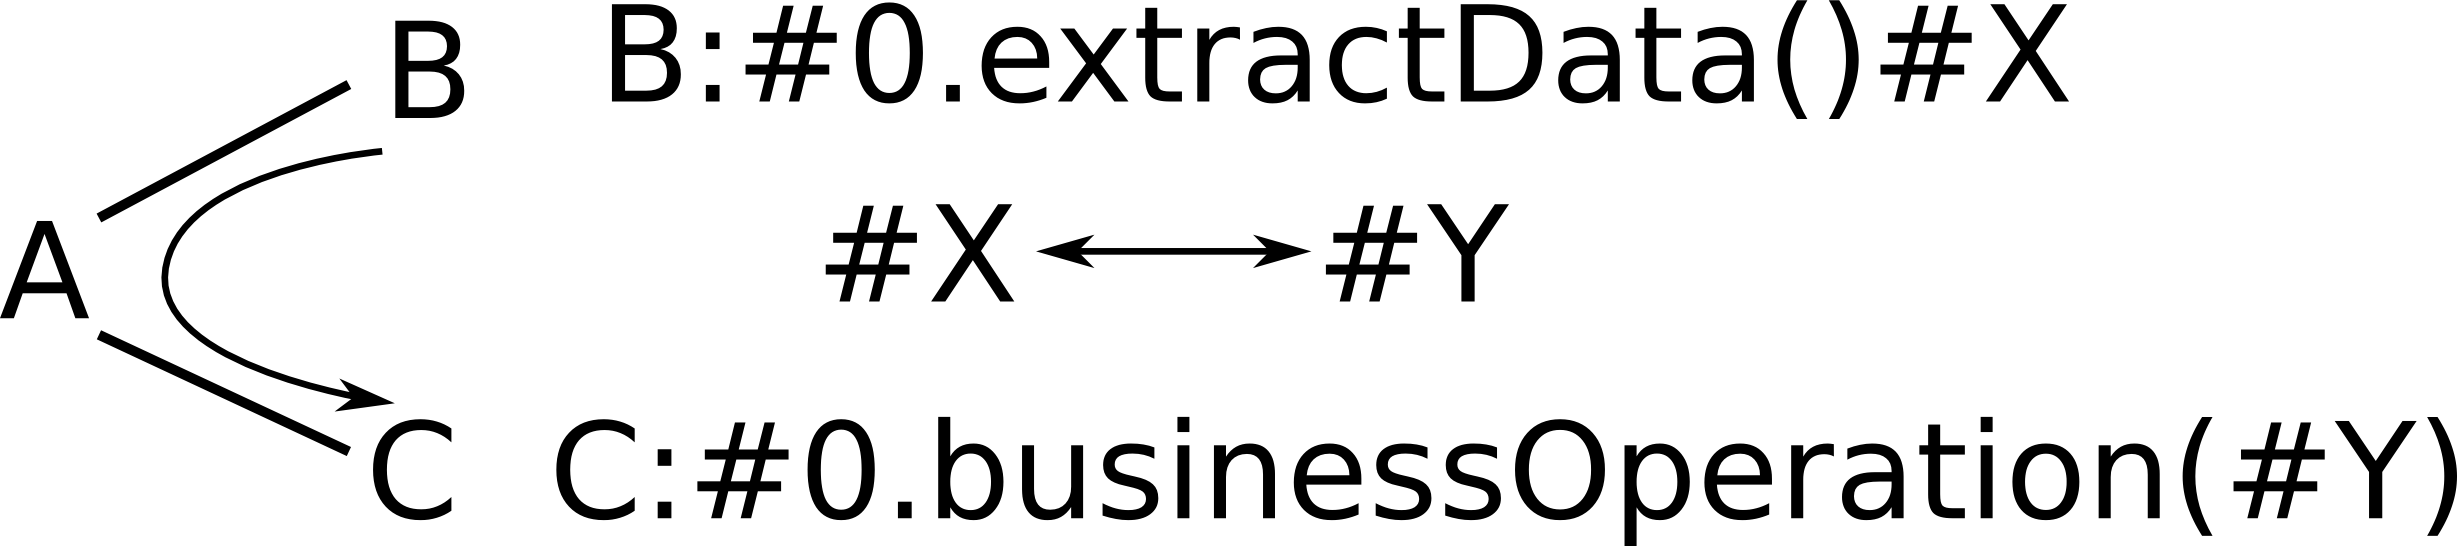
\includegraphics[width=1\textwidth]{logicGarbageSimpleSolutionFig}
\end{figure}
\end{frame}

% \begin{frame}{Problem - Paskudne zaśmiecenie logiki}
% ABnCn Rysunek z rozwiązaniem dla wiele warstw
% \end{frame}


\subsection{Demo}
\begin{frame}{Demo}
 DEMO
\end{frame}

\section{Argumentacja}

\begin{frame}{Czy naprawdę warto??}
 Masło maślane?

\hfill

\pause

Why Functional Programming Matters - John Hughes 1984

\hfill

Modular design $+$ Glue $\Rightarrow$ Complex systems

\pause

\hfill

Programowanie funkcyjne daje nowe narzędzia:
\begin{enumerate}
 \item Funkcje wyższego rzędu 
 \item Lazy evaluation
\end{enumerate}

\end{frame}

\begin{frame}{Moduły jako funkcje}
 Rysunek
\end{frame}

\begin{frame}{Lazy evaluation}
 Rysunek
\end{frame}


\begin{frame}{Plany}
``Program napisane przez jedną osobę to mały program. Inaczej by się nie udało''.

\textbf{Filip Murlak}
\end{frame}

\begin{frame}{Plany}

Plan: Napisać mały program, który pomoże zrobić duże.

 \begin{enumerate}
  \item<2-> Implementacja rozproszona
  \item<3-> Test przeciążenia - warsztaty bez ograniczeń na ilości osób
  \item<4-> Injection Bus
 \end{enumerate}
\end{frame}

\section{Pytania}
\begin{frame}{Pytania}
Pytania?????
\end{frame}

\begin{frame}{Pytania}
Pytania:
\begin{enumerate}
 \item<1-> Garbage collector ????
 \item<2-> Zmiana kontekstu transakcji ????
 \item<3-> Wyjątki ????
 \item<4-> Call reorder - formal specification ????
\end{enumerate}

\end{frame}






\end{document}
